\section{Methodology}
\label{s:methodology}
In this section several points regarding the methodology used in the work will be presented. The general approach taken to modeling, as well as the models themselves will be explained. The metrics used to evaluate the goodness of fit of the different models will also be presented. 

\subsection{Overview of modeling approach}
In order to understand why the models that will be presented below have been chosen and why the evaluation metrics have been chosen, it is worth first taking a look at the requirements of the modeling task and the general criteria that determine what a good result is.

\subsubsection{Modeling task characteristics}
\label{s:modeling-task-characteristics}
The general technical characteristics of the task, from the objectives and the time series characteristics already explored are the following:
\begin{itemize}
    \item \textbf{Modeling horizon}: The horizon to be modeled is of between 1 and 10 years, or between 8.760 and 87.600 hourly time steps. 
    \item \textbf{Available data}: The data available for the training and testing tasks consists of slightly below 10 years of data, or slightly below 87.600 observations. This data has been consistently recorded at a 1-hour time step interval.
    \item \textbf{Seasonality}: There has been found to be high seasonality, both at the daily and yearly frequencies. 
    \item \textbf{Exogenous variables}: A certain predictive power of some series with respect to the others has been found. Thus, the capacity of incorporating the use of exogenous variables or multivariate modeling approaches are specially interesting. 
    \item \textbf{Extreme values}: There is a special interest in having accurate modeling of the extreme values, specially in the wind capacity factor.
    \item \textbf{Point wise forecast}: The forecasts produced by the model can be point wise predictions, there is no need to produce probabilistic forecasts for each time step.
\end{itemize}

\subsubsection{Modeling criteria}
Starting with the objectives already outlined in the section called \nameref{sec:objective-and-scope}, here these objectives will be broken down into more specific criteria that the best model must aim to meet in the best possible way. The specific characteristics the model must meet are the following:
\begin{itemize}
    \item \textbf{Seasonality}: The chosen models must be able of incorporating seasonality into its forecast. 
    \item \textbf{Multiple variables}: The chosen models should be able to incorporate multiple variables, be it through a multivariate modeling, through historical exogenous variables and/or through future exogenous variables. Through the modeling task it will be made apparent whether incorporating the information of the other series helps in modeling a given series.
    \item \textbf{Complex relationships}: The temporal relationships of a series with itself and the relationships of a series with the other variables are probably more complex than linear relationships. That is why a model capable of incorporating complex non-linear temporal and intervariate relationships will probably have an advantage.
    \item \textbf{Multiperiod modeling}: As it has already been mentioned, the modeling period will encompass between 8.760 and 87.600 time steps. The model must be able to create such forecasts. But going further, if the prediction is created by autoregressively estimating the next step, there is a compounding in errors over time \cite{educing_error_propagation_long}. By estimating multiple time steps in one prediction pass, the number of autoregressive steps can be reduced and with it the compounding of errors can be reduced too. Therefore, models with bigger single-step prediction window should have an advantage.
    \item \textbf{Long and short term temporal relationships}: The model must be able to incorporate both long term and short term temporal relationships.
    \item \textbf{Robustness}: The model must be resistant to overfitting, given the parameter size of some models and the number of available training data points. 
    \item \textbf{Extreme value accuracy}: The model must be specially sensitive to extreme values, be it through the flexibility of incorporating a custom loss function or through its intrinsic characteristics.
    \item \textbf{Computational efficiency}: Given the long modeling horizon, the model must be efficient both in prediction time and in memory used when training and when incorporating historical data in prediction.
\end{itemize}
\subsection{Models}
\label{s:models}
Now that the criteria used to select potential models has been outlined, the different models that will be evaluated can be presented. These models have been divided by model family or type. Here below, the different model types and each of the models and their characteristics and main working principles are explained. 
\subsubsection{Statistical models}
These models are based on classical statistical methods to analyze and predict temporal series. They use techniques like regression analysis, autocorrelation and spectral analysis to model and forecast temporal variables. The ones that will be used here are:
\begin{itemize}
    \item \textbf{Linear Regression}: This is the simplest model and it will be used as a naive benchmark. It models a given capacity factor value for one of the series as a linear combination of several exogenous variables. In this case, those variables are the values of Fourier sine and cosine terms, some lagged values of the given time series and some lagged values of other time series, which in this case will be the other capacity factors. The main parameters of the model are thus:
    \begin{itemize}
        \item Seasonal frequencies: That is the frequencies for which the Fourier terms will be calculated. It can be daily, yearly, both, etc.
        \item Fourier harmonics: For each of the seasonalities, several harmonics of Fourier terms can be calculated, creating more nuanced patterns the more harmonics are added.
        \item Autoregressive order: That is, what lags of the modeled series to incorporate.
        \item Exogenous lags: That is, what lags of the other two series to incorporate. 
    \end{itemize}
    The mathematical formulation for the model thus is:
    \begin{multline}
        Y_t=\beta_0 + \sum_{\tau}\sum_{k}\left[\gamma_{\tau,k}\sin\left(\frac{2\pi k t}{\tau}\right) + \delta_{\tau,k}\cos\left(\frac{2\pi k t}{\tau}\right)\right] +\\+ \sum_l \phi_l Y_{t-l} + \sum_v\sum_p\theta_{v,p}X_{v,t-p} + \epsilon_t
    \end{multline}
    where $\tau$ is each of the seasonality periods, $k$ is each of the fourier harmonics, $l$ is each of the self lags, $v$ is each of the other two capacity factors and $p$ is each of the lags used for the two other capacity factors.
    
    This model operates on several assumptions which are worth mentioning. The first is that all relationships -- those with the seasonal terms, with lagged values, with the other capacity factors, etc. -- are assumed to be linear. The error term $\epsilon_t$ is assumed to be independent and identically distributed (i.i.d.) with constant variance (homocedastic) and Gaussian, although there is no evidence that this is true for the three modeled series. That is why the Box-Cox transform is used before fitting the model.
    \item \textbf{ARIMAX}: The AutoRegressive Integrated Moving Average with eXogenous variables model is an extension to the previous model. It incorporates both autoregressive and moving average components to the endogenous time series and allows for time  integration, which extends the purely autoregressive view in the previous model, as well as some exogenous variables. It provides a more complex representation of the relationship of the time series with its lagged values than the linear regression model presented above. To the previously presented parameter, these new ones are added:
    \begin{itemize}
        \item Integration order: This represents the number of times the endogenous time series is differentiated. 
        \item Moving average order: That is, what moving average error terms are incorporated.
    \end{itemize}  
    The new model formulation is:
    \begin{multline}
        Y_t=-\left(\Delta^d Y_t - Y_t\right) + \beta_0 + \sum_{\tau}\sum_{k}\left[\gamma_{\tau,k}\sin\left(\frac{2\pi k t}{\tau}\right) + \delta_{\tau,k}\cos\left(\frac{2\pi k t}{\tau}\right)\right] +\\+ \sum_l \phi_l \Delta^d Y_{t-l} + \sum_q \theta_q \epsilon_{t-q} + \sum_v\sum_p\theta_{v,p}X_{v,t-p} + \epsilon_t
    \end{multline}
    where $d$ is the order of differentiation with $\Delta Y_t = Y_t - Y_{t-1}$ and $q$ is lags of the error term added for the moving average.
    \item \textbf{VARMAX}: The Vector AutoRegressive Moving Average with eXogenous variables is a modification of the ARIMAX model, but without the integration component and turning the single variable endogenous variable into a vector variable. This model jointly predicts all capacity factor variables, directly creating the joint distribution. The model is formulated as:
    \begin{multline}
        Y_t= \beta_0 + \sum_{\tau}\sum_{k}\left[\gamma_{\tau,k}\sin\left(\frac{2\pi k t}{\tau}\right) + \delta_{\tau,k}\cos\left(\frac{2\pi k t}{\tau}\right)\right] +\\+ \sum_l \phi_l Y_{t-l} + \sum_q \theta_q \epsilon_{t-q} + \epsilon_t
    \end{multline}
    where $Y_t$ here is not a single variable data point but a three-dimensional vector containing all three capacity factors. The coefficients are also vector coefficients.
\end{itemize}

\subsubsection{Machine Learning models}
Machine learning models are a class of models designed to learn more complex patterns from data with less constraining assumptions and generally more parameters. Even if these models are quite general and are not specifically designed for time series modeling, they can be readily used for this purpose. For this specific use case, these models excel at capturing complex and non-linear relationships that statistical methods may overlook, they can therefore outperform the former methods when these characteristics are present or when data is highly non-stationary or with intricate dependencies. The ones that have been implemented are:
\begin{itemize}
    \item \textbf{SVM}: Support Vector Machines introduced in \cite{cortes_vladimir_vapnik_1995} are ML models that can be used for either classification or regression. They work by finding the optimal hyperplane that separates the data points into distinct classes or predicts values with the maximum margin. In the specific case of regression the model is known as Support Vector Regression (SVR). Its objective is to find a function $f(x)$ that deviates from the empirical values $y_i$ by at most a margin $\epsilon$ ensuring the model remains as flat as possible. That is, preventing overfitting. The function takes the form:
    \begin{equation}
        f(x)=w^T\phi(x)+b
    \end{equation} 
    where $w$ is the weight vector, $b$ is the bias term and $\phi(x)$ is a transformation that maps the input data into a higher-dimensional space. The SVR algorithm solves the following optimization problem:
    \begin{equation}
        \begin{aligned}
            \min_{w,\xi_i,\xi_i^*} \quad & \frac{1}{2}\|w\|^2+C\sum_{i=1}^n\left(\xi_i+\xi_i^*\right)\\
            \textrm{s.t.} \quad & y_i-f(x_i) \leq \epsilon+\xi_i\\
            & f(x_i)-y_i \leq \epsilon + \xi_i^*\\
            & \xi_i,\xi_i^*\geq 0
        \end{aligned}
    \end{equation}
    where $\xi_i$ and $\xi_i^*$ are slack terms allowing for some flexibility in prediction errors and $C$ is the regularization parameter that controls the trade off between the flatness of the function and how well it fits the data. Solving the optimization problem provides:
    \begin{equation}
        f(x) = \sum_{i=1}^n\left(\alpha_i-\alpha_i^*\right)K(x_i,x)+b
    \end{equation}
    where $\alpha_i$ and $\alpha_i^*$ are the optimal Lagrange multipliers corresponding to the slack variables $\xi_i$ and $\xi_i^*$ and $K(\cdot)$ is the Kernel function used to calculate the distance between predicted and empirical data points and which provides the needed non linearities to the function. In this case, the Radial Basis Function has been used with 
    \begin{equation}
        K(x_i,x_j)=e^{-\gamma\|x_i-x_j\|^2}
    \end{equation}
    where $\gamma$ controls the spread of the kernel.

    As it can be seen, the SVR is quite useful as it includes non-linear relationships, has built in robustness to overfitting and is quite scalable. However, it is quite sensitive to the choice of parameters -- mainly that of kernel, $C$ and $\epsilon$ -- and assumes the relationship between input space and prediction remains constant in time, so it is not that appropriate for non-stationary time series. 

    In the implementation used in this work, the input space is equivalent to that of the classical statistical models, comprised of some lags of the data, some Fourier decompositions at different levels and some lags of the other time series. 
    \item \textbf{XGBoost}: eXtreme Gradient Boosting introduced by \cite{chen_guestrin_2016} is a highly efficient and scalable implementation within the paradigm of decision trees. Decision trees are another ML framework where starting from a root node, the dataset or output space is split into two or more subsets based on a specific value of a selected feature. For example, a very simple example would be to say that on average the predicted solar capacity factor is 0.3 (root node). If it is daytime the predicted value is 0.6 and if it is nighttime the predicted value is 0.0 (two subsequent nodes). This split can be further refined with more levels on different values of different features, providing a more accurate and non-linear prediction based on the input values. Trees are built through an algorithm which at each node selects the feature that best separates the data based on a criterion such as entropy. This model is quite simple but allows for non-linearity and is very robust to different scales in input features. However, it can easily overfit on the training data and the results can be quite unstable. 
    
    Returning to XGBoost, this model builds sequential trees where each new tree corrects the errors of the previous one in what is known as an ensemble of trees. It also implements several improvements such as regularization, tree pruning or parallelization. The model thus builds a prediction like
    \begin{equation}
        \hat{y}_i^{(t)} = \hat{y}_i^{(t-1)} + f_t(x_i)
    \end{equation}
    where $\hat{y}_i^{(t)}$ is the prediction after $t$ trees and $f_t(\cdot)$ is the tree added at level $t$. Each individual tree is constructed optimizing an objective function which both minimizes the loss function between true and predicted value and also has a regularization term which prevents overfitting. The objective thus becomes
    \begin{equation}
        \min_\theta \sum_{i=1}^n L(y_i,\hat{y}_i) + \sum_{k=1}^K \Omega(f_k)
    \end{equation}
    with the regularization term for each tree $k$ being 
    \begin{equation}
        \Omega(f_k)=\gamma T + \frac{1}{2}\lambda\sum_{j=1}^{T}w_j^2
    \end{equation}
    with $T$ being the number of nodes in the tree, $w_j$ being the weight of leaf $j$ and $\gamma$ and $\lambda$ being regularization parameters.

    This model has some of the same advantages as the ability of capturing non-linear relationships and built in regularization, but it also allows for some features like custom loss functions.
    
    In the implementation used for the XGboost, the input space is again equivalent to that of the classical statistical models with some lags of the data, some Fourier decompositions at different levels and some lags of the other time series. 
\end{itemize}

\subsubsection{Neural Network models}
Neural networks are computational models inspired by the brain's morphology. They are formed by \textit{neurons}, which are the basic unit which take several weighted inputs, sums them and adds some bias and applies an activation function which provides the non linearities in the model. Many of these neurons are connected across several layers, and end up providing a final prediction. For each layer, the mathematical expression can be represented as
\begin{equation}
    A=\sigma\left(WX+B\right)
\end{equation}
where $A$ is the output of the layer, $X$ is the input vector, resulting from the previous layer or the input itself, $W$ is the weight vector, $B$ is the bias and $\sigma(\cdot)$ is the activation function to be applied element wise to the resulting vector. This function can be a ReLU, tanh or sigmoid among others. 

Neural networks have been shown to be universal approximators by \cite{hornik_stinchcombe_white_1989}, meaning that any arbitrary function can be perfectly approximated by a feedforward neural network with at least one hidden layer. In practice however there is hardly enough data to provide such an approximation and overfitting is quite easy due to the number of parameters. This has lead to the appearance of many NN architectures, trying to adapt them to specific use cases. These are the NN models that have been implemented for this work. 
\begin{itemize}
    % \item \textbf{LSTM}: Long-Short Term Memory NN are a specific architecture of NN that instead of using the previously explained neurons use a more complex type of basic unit called memory cells. These memory cells can maintain and update information over time using gates that control the flow of information. The basic structure of the LSTM can be seen in the following diagram:
    % \begin{figure}[ht]
    %     \centering
    %     \captionsetup{justification=centering}
    %     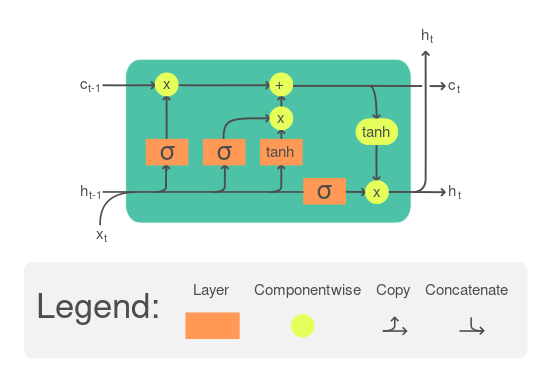
\includegraphics[width=0.7\linewidth]{assets/LSTM_Cell.png}
    %     \caption{LSTM memory cell}
    %     \label{fig:lstm-memory-cell}
    % \end{figure}
    % In \autoref{fig:lstm-memory-cell}, $x_t$ is the input vector, $h_t$ is the hidden state vector and $c_t$ is the cell state vector. Each of the layers in the figure's legend or gates have a feedforward network architecture with its weights and biases. The forget gate decides what information to discard from the previous state, the input gate decides which pieces of new information to store in the current cell state and the output gate controls which pieces of information in the current cell state to output. The cell state remembers values over arbitrary time intervals. Over training, the parameters of the different gates are adjusted. 

    % LSTM networks can thus retain temporal relationships over arbitrary lengths. They were developed in \cite{hochreiter_schmidhuber_1997} as an alternative to Recurrent Neural Networks (RNN). These are a simpler NN architecture designed to handle sequential data, which through a series of feedback connections are allowed to retain information about previous states. RNN however have some computational issues commonly referred to as the vanishing gradient problem which prevents them from learning after a certain point. This issue is solved through the LSTM architecture. It also has some other quite useful characteristics such as also being able to model complex non linear relationships with more freedom than other classical ML models and can also provide multi step forecasting, allowing for modeling of a certain period in less steps. 

    % The input vector again contains lags of the modeled series and the other two series as well as fourier decomposition components. 

    % The main issue with LSTM is however its much higher computational complexity compared with simpler models, as well as needing large amounts of data and being more prone to overfitting than other simpler models. 
    
    \item \textbf{N-BEATS}: The Neural Basis Expansion Analysis for interpretable Time Series forecasting is another relatively new NN architecture focused on time series modeling through deep learning, mainly on the univariate case. Its architecture can be summarized through the following diagram obtained from the mentioned paper:
    \begin{figure}[ht]
        \centering
        \captionsetup{justification=centering}
        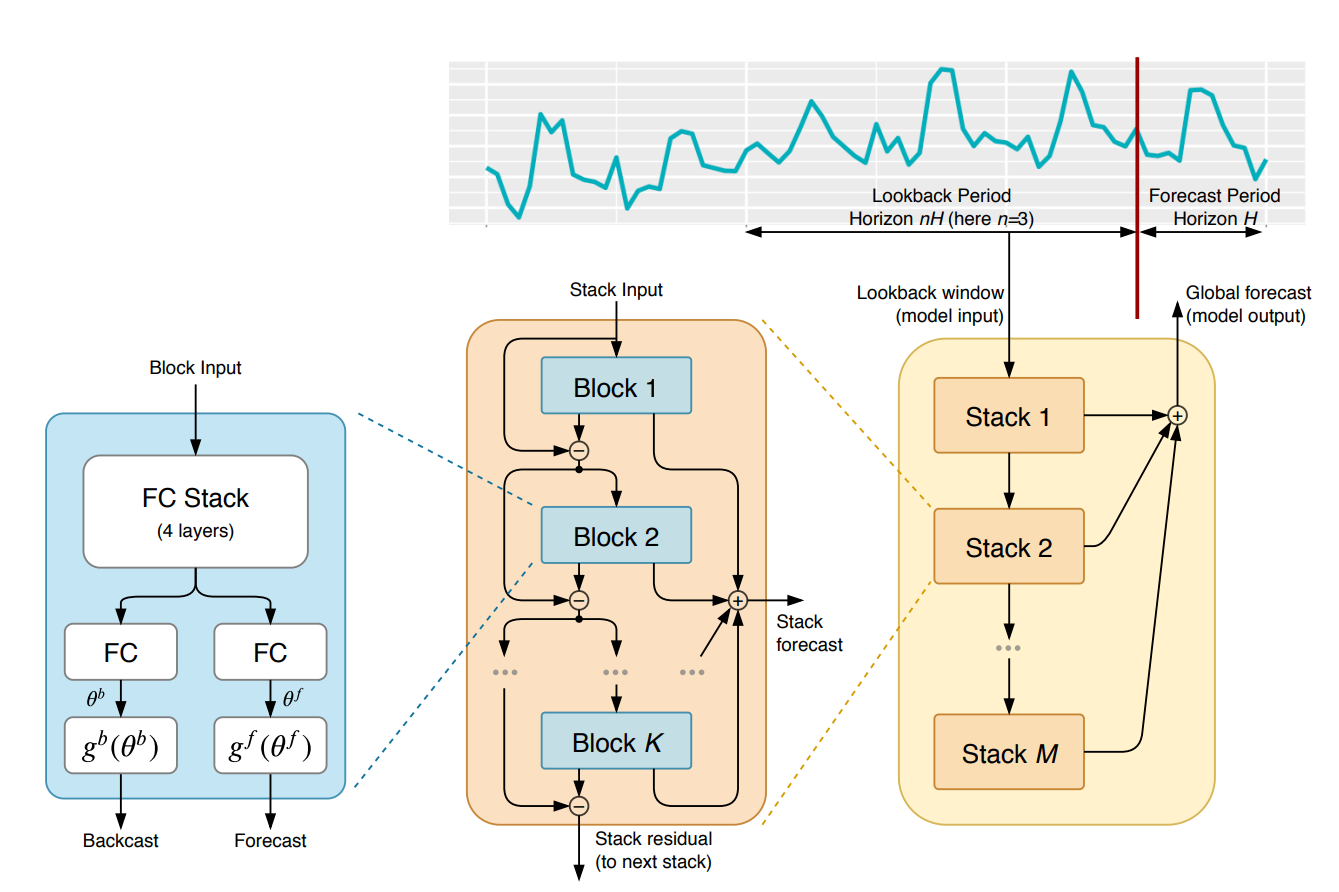
\includegraphics[width=\linewidth]{assets/nbeats-architecture.png}
        \caption{N-BEATS architecture}
        \label{fig:nbeats-architecture}
    \end{figure}
    Through \autoref{fig:nbeats-architecture} it can be seen how the model works. There are several stacks, each created by blocks of fully connected feedforward networks. Each block predicts a part of the forecast with the information from the lookback period. The fully connected stack in the block predicts both the forecast and the backcast -- data in the lookback period. The backcast is subtracted to the previously available lookback period, so each block tries to model the forecast from the residuals of the previous block in a very similar way to how each of the trees in the XGBoost predicts the error of the previous tree. The output of each of the blocks is summed to create the stack output, and all the stack's outputs is aggregated to create the final forecast. This architecture is supposed to automatically decompose the time series into different components like trend and seasonality in an interpretable way. This model has demonstrated state-of-the-art performance in several time series benchmarks such as the M3 and M4. It is also domain agnostic, making no assumptions on stationarity or seasonality and it works well without any feature engineering. The training is also more efficient than for an LSTM, as the lack of recurrent feedback loops allows for parallelization of the training. It also allows for a multistep forecasting window. 
    
    \item \textbf{N-HiTS}: The Neural Hierarchical Interpolation for Time Series forecasting is another quite a recent architecture developed by \cite{challu_olivares_oreshkin_garza_2022}. It was developed with the explicit goal of modeling long term relationships in time series data in a more memory and computation efficient way. The architecture overview can be seen in the following diagram, obtained from the mentioned paper:
    \begin{figure}[ht]
        \centering
        \captionsetup{justification=centering}
        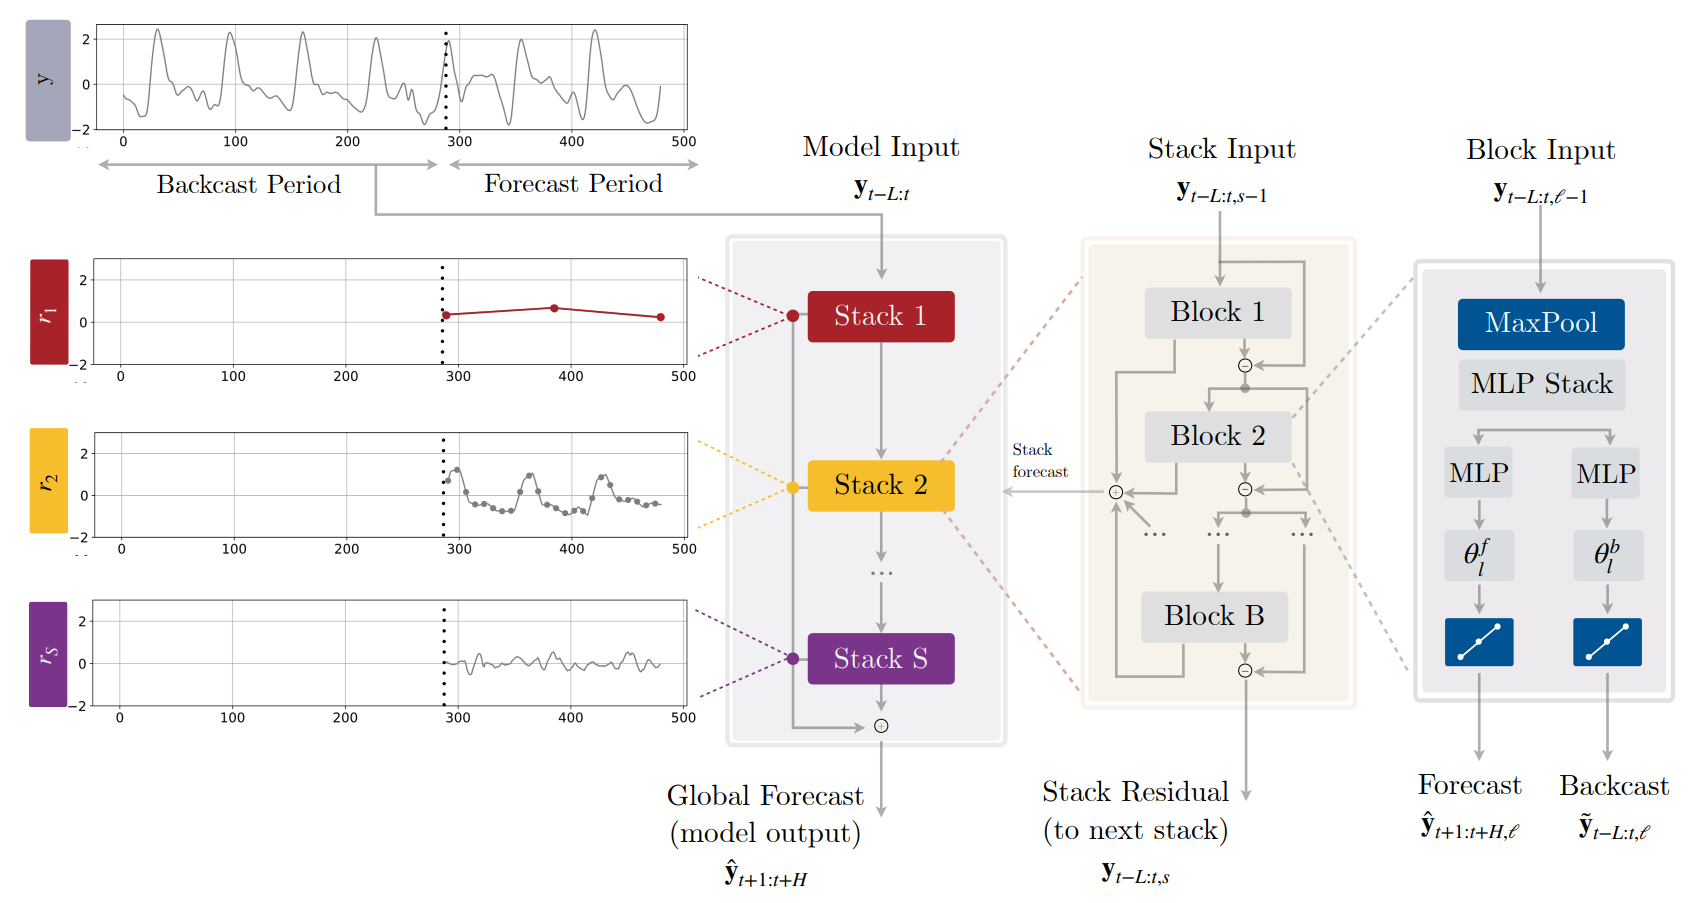
\includegraphics[width=\linewidth]{assets/nhits-architecture.png}
        \caption{N-HiTS architecture}
        \label{fig:nhits-architecture}
    \end{figure}
    As it can be seen in \autoref{fig:nhits-architecture}, the architecture is quite similar to the N-BEATS model with some added complexity. The model works first by sampling the historical window used in forecasting at different frequencies. Then, a series of MLP (feedforward NN) stacks are used in an ensemble way to forecast the following data point at each of the different forecasting frequencies. In the ensemble, each of the MLP stacks produces a prediction of the historic data which is subtracted from the previous historic data, so each MLP block exclusively tries to approximate the residuals of the previous one -- very similarly to how each tree reduced the error of the previous tree in the XGBoost model. Then, the predictions across all frequencies are interpolated to provide a prediction for each of the minimal frequency data points. 
    
    This architecture allows each stack to focus on capturing the relationships at a different frequency, and it does it in a very efficient way, not really needing all data points for all relationships. This allows for very good performance in several long term time series as shown in the mentioned paper. Even if this is exclusively a univariate model, it has been shown to outperform several state of the art multivariate models. It remains to be seen however if following an exclusively univariate effect the cross relationships between all three series can be maintained.
    
    Also note how given the architecture, in this case it is not necessary to explicitly include time related variables such as the Fourier decompositions as inputs, as these relationships are automatically learned through the different frequencies' sampling.

    \item \textbf{TimeMixer}: The TimeMixer model was prpoposed by \cite{wang_wu_shi_hu_luo_ma_zhang_zhou} in 2024. This MLP architecture leverages the idea that time series present different patters for different sampling scales. It mixes information across different time steps in a much more efficient way than other sequential models like LSTM or attention based models. The TimeMixer model has Past-Decomposable-Mixing (PDM) blocks which for different resolutions extracts the trend and seasonal components -- through bottom up and top down mixing respectively. After several PDM blocks, each of the different scales has different information with different prediction capabilities. Thus, a Future-Multipredictor-Mixing block combines the predictions of these different scales. The FMM can be thus understood as an ensemble of multiple predictors where each predictor leverages the information of a different scale. This is probably better understood through the diagram presented by the authors in the paper.
    \begin{figure}[ht]
        \centering
        \captionsetup{justification=centering}
        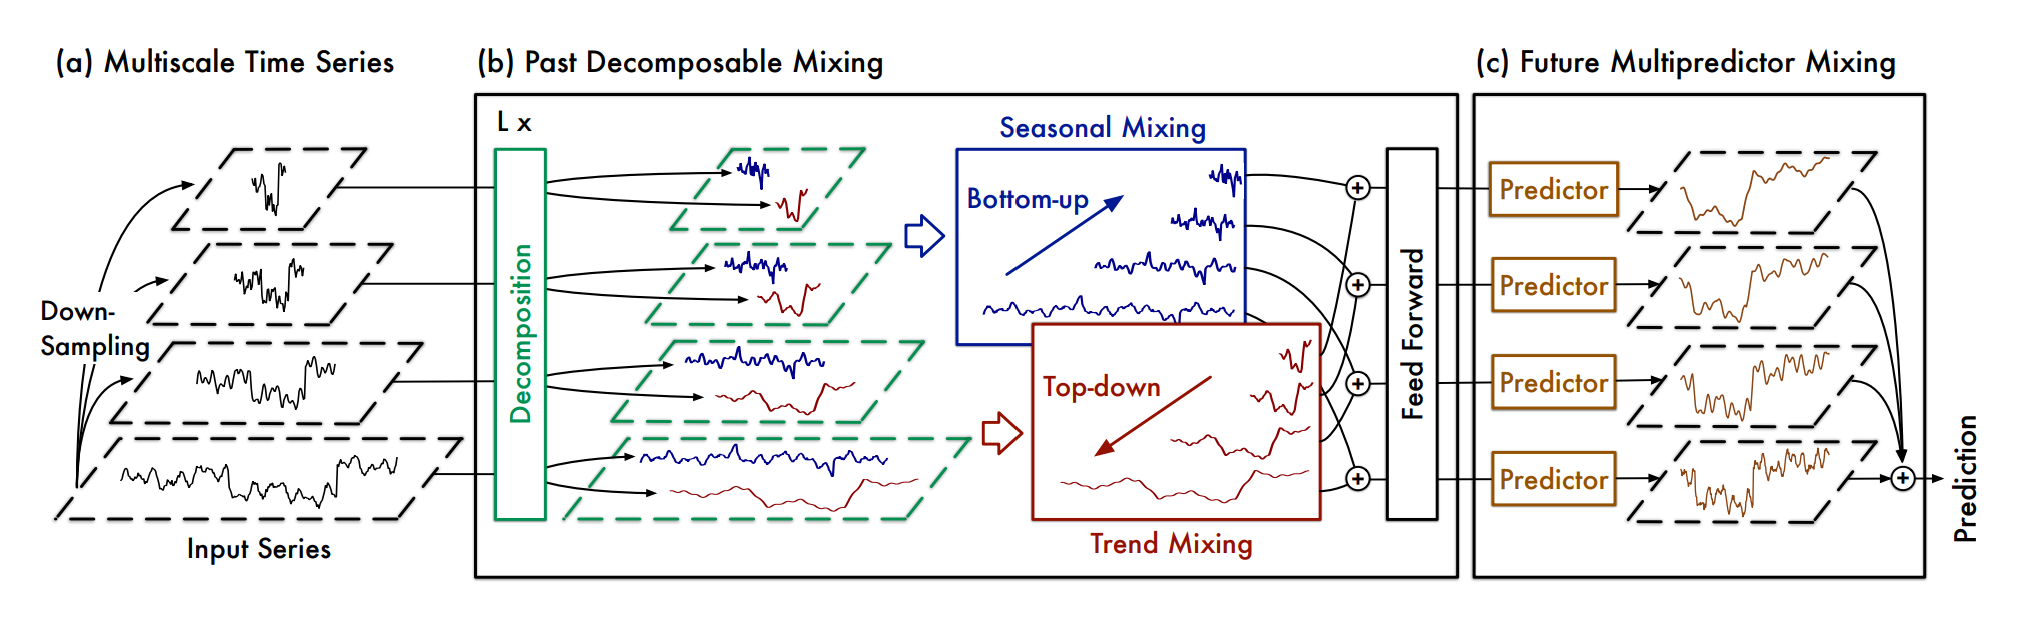
\includegraphics[width=\linewidth]{assets/timemixer-architecture.png}
        \caption{TimeMixer simplified architecture}
        \label{fig:timemixer-architecture}
    \end{figure}
    This architecture is furthermore inherently multivariate, also mixing information across different variables and thus capturing their interactions. Additionally, thanks to its MLP based architecture it is very computationally efficient compared to other recurrent or attention based models, being capable of having longer input sequences and faster training and execution times. 
\end{itemize}
\subsubsection{Transformer models}
Transformers are in reality also a type of deep learning or NN model. However, it incorporates a series of new key components that make it different enough to merit its own category. Introduced by \cite{vaswani_2017} in the legendary \textit{Attention is All You Need} paper that sparked the LLM revolution, the transformer architecture is a NN architecture that incorporates a self-attention mechanism used to process data. This self-attention mechanism is in simple terms a way of weighting the importance of different elements in a sequence relative to each other. This allows for a weighted sum of the input sequence focusing on relevant past information. It also contains other key components like the Positional Encoding, which is added to the input sequence to provide information about the position of each element in the such sequence. This general architecture is immensely flexible and has been applied successfully to many problems, most notably to natural language generation. This basic model has also sparked a series of subsequent models with some modifications that make them specially suited for some tasks such as time series modeling. The architectures used in this work are:
\begin{itemize}
    \item \textbf{TFT}: Temporal Fusion Transformers introduced by \cite{lim_arık_loeff_pfister_2021} are a specific implementation of the transformer architecture used for time series modeling. It has three main components. The first is a set of Variable Selection Networks (VSN) which select the most relevant input variables. These can be static variables, dynamic historically known variables or dynamic generally known variables -- where not only the past values are known, but future values are also known. The selected input goes into an LSTM based encoder which captures short term dependencies. Finally, a self-attention based decoder captures long term dependencies using transformers. All of this is coordinated through different gating mechanisms that modulate the flow of information between the different layers. A final key feature of this architecture is its in built ability to produce quantile forecasts. This however will not be specially useful for the task at hand. A more in depth overview of the architecture can be seen in \autoref{fig:tft-architecture}, obtained from the aforementioned paper. 
    \begin{figure}[ht]
        \centering
        \captionsetup{justification=centering}
        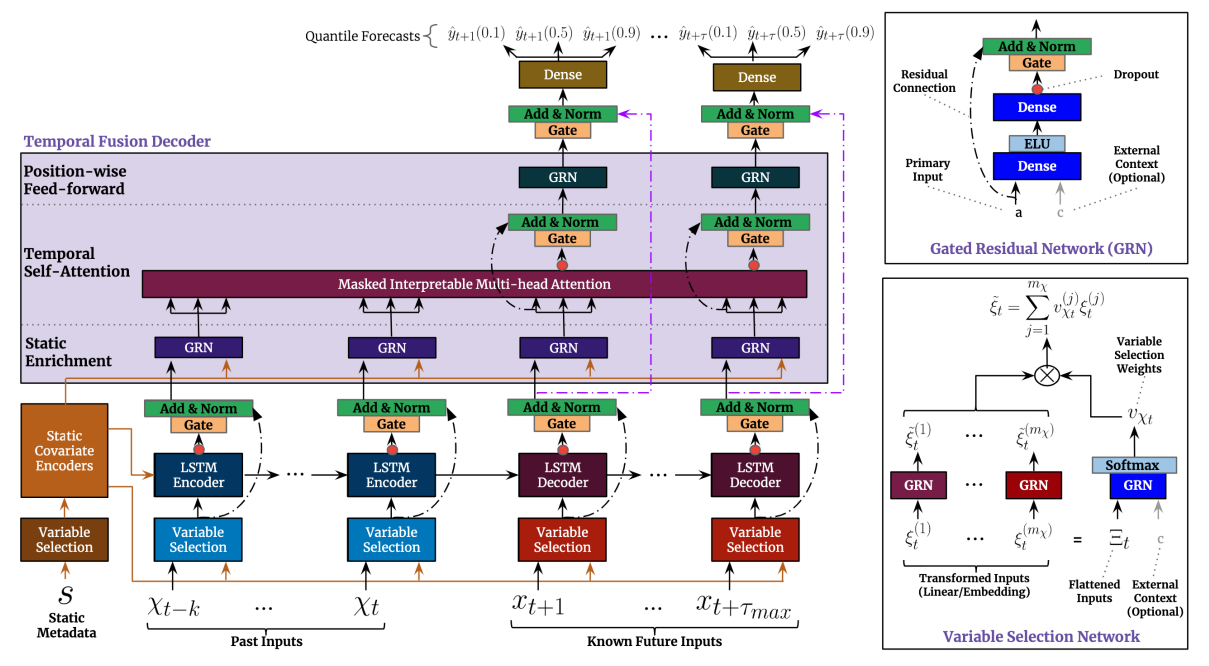
\includegraphics[width=\linewidth]{assets/tft-architecture.png}
        \caption{TFT architecture}
        \label{fig:tft-architecture}
    \end{figure}
    The TFT architecture has some very interesting features like explicitly capturing short and long term dependencies, regularization through the gating mechanisms, multistep prediction or interpretability of variable importance. However, this comes at the expense of high computational cost, high model complexity and high data requirements.
    \item \textbf{Informer}: A different transformer based architecture developed by \cite{zhou_zhang_peng_zhang_li_xiong_zhang_2021} specifically developed for forecasting of long sequence time-series through a more efficient implementation. The main advances introduced in this model are the use of a \textit{ProbSparse} self-attention mechanism which has a time and memory complexity of $\mathcal{O}(n\log n)$ instead of $\mathcal{O}\left(n^2\right)$ -- with $n$ being the lookback period --, a decoder which predicts the long time-series sequence in one operation rather than step by step and an input method specifically developed to handle extremely long input sequences. 
    
    The Informer has many of the same benefits of other transformer based architectures, but with the added feature of being more efficient and thus being able to incorporate a longer lookback period and thus capturing longer range dependencies that may escape some other architectures. All the while being also more efficient at inference time and thus faster in formulating predictions. However, it also shares many of the same disadvantages of other transformer based models like requiring vast amounts of data for proper training or being very resource intensive, even with the added efficiency.  
    \item \textbf{FEDFormer}: The Frequency Enhanced Decomposed Transformer presented by \cite{zhou_ma_wen_wang_sun_jin_2022} is yet another transformer based architecture specially designed for long sequence time series modeling. It leverages a principle similar to the N-HiTS. It uses the idea that complex time series have a much more compact representation in the frequency domain, which also captures both long term trends and shorter term seasonal components. To act upon this principle, the authors make several changes to the base transformer architecture, substituting the Multi-Headed Self-Attention block with a Frequency Enhanced Block and the Multi-Headed Cross-Attention block with a Frequency Enhanced Attention block. Both of these leverage Fourier transforms within their operations to operate on the frequency domain. However, the authors also provide the option of using the Wavelet Transform (WT) instead of the Fourier Transform (FT). Using the WT which transforms the input to the frequency and time domain, not only to the frequency domain as the FT, allows for a more nuanced although complex representation of the input data. For this work, the FT implementation will be used due to its simpler implementation. 
    
    Altering the transformer to operate on the frequency domain also has as a consequence reducing the complexity further down even from the Informer to linear time and memory. 
    
    Apart from accentuating the benefits already mentioned in the Informer, in the paper it is demonstrated how the predicted distribution is closer to the ground truth distribution according to the Kolmogorov-Smirnov distribution test, which is a specially interesting characteristic given the work objectives and evaluation metrics explained in \autoref{s:evaluation-metrics}.

    \item \textbf{iTransformer}: The inverted Transformer model introduced by \cite{liu_hu_zhang_wu_wang_ma_long_2023} is another novel architecture based on transformers which is inherently multivariate. To understand its innovations it is convenient to first understand how normal multivariate transformers work. These transformers take the multivariate time series and slice it temporally. Each token is thus a given timestamp with each of the variable's values. The iTransformer takes the opposite approach. Instead of splitting the time series temporally and embedding each of the time steps, it splits the time series per variable and embeds these variables. The attention mechanism is then run on the variate tokens instead of the temporal tokens. The feedforward network then is run on the time series representation, while in traditional transformers it is run on the multivariate representation. To better understand this concept it an be useful to look at \autoref{fig:transformer-vs-itransformer} obtained from the mentioned paper.
    \begin{figure}[ht]
        \centering
        \captionsetup{justification=centering}
        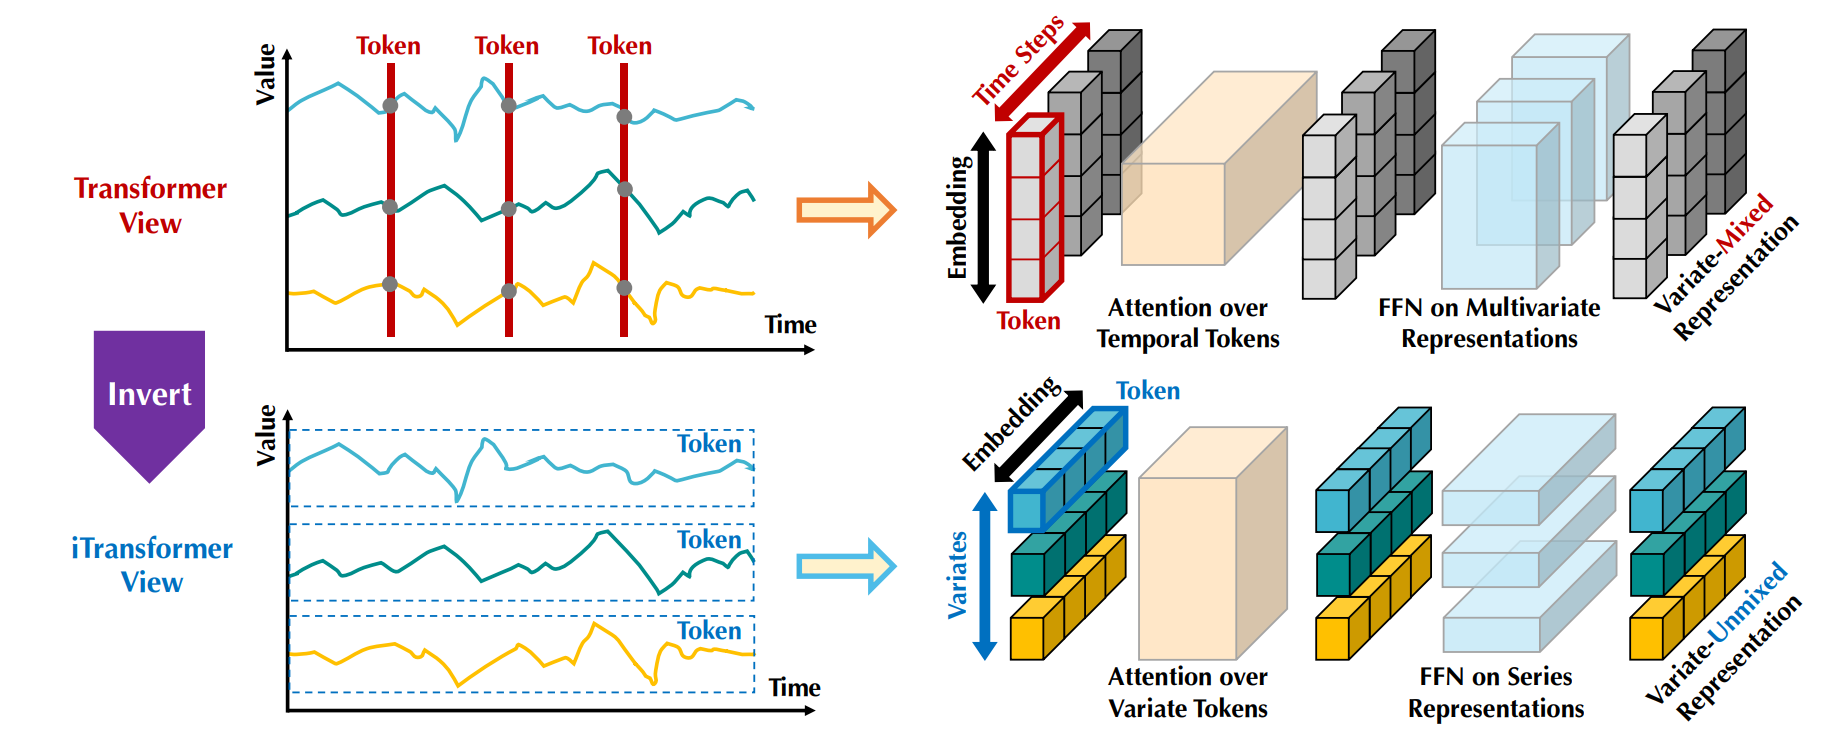
\includegraphics[width=\linewidth]{assets/transformer-vs-itransformer.png}
        \caption{Comparison of traditional transformer and inverted transformer embedding and general architecture}
        \label{fig:transformer-vs-itransformer}
    \end{figure}
    Through this change in architecture, the iTransformer gains some benefits with respect to the traditional transformer. It has been observed that for traditional transformers increasing the lookback period does not necessarily translate to better evaluation metrics due in theory to the \textit{distraction} of the attention mechanism, however by leveraging the MLPs on the temporal dimension the iTransformer can gain more benefit from extended lookback periods. Its architecture also allows for seamless multivariate modeling, allowing it to even better generalize to unseen variables and to easily change the number of variables included in the modeling. In general, the inverted architecture achieves a better performance in most benchmarks as presented not only in the mentioned paper, but also in independent benchmarks like \cite{wang2024tssurvey} where the iTransformer is the best performing model for long term forecasting with shared hyperparameters out of the 15 evaluated transformer and NN based models.

    It is worth noting how the inverted architecture can be applied to most transformer models, including the ones used here. It is possible for example to create an iInformer model by inverting the dimensions of transformer mechanism in the Informer model. Here however the iTransformer model used is the inverted vanilla transformer architecture, in order to not confound performance with other improvements added by other architectures. 
\end{itemize}
\subsubsection{Comparison}
After having presented all model classes and the different models that will be implemented themselves, it can be useful to perform a quick comparison and an a priori judgement of which models should outperform the rest, even if all of them will be implemented and evaluated. 

It can be seen how there is a very wide range of models from which to choose from -- many more than the ones presented here. It is worth noting how here only the base models have been analyzed, and no custom combinations between them have been explored. These combinations can be very useful in combining useful characteristics of two or more base models and creating more accurate predictions as shown in \cite{zou_yang_2004}.

Out of all models here analyzed, it would seem like the most appropriate due to its intrinsic characteristics is the FEDFormer due to it being able to include a very long forecasting horizon and lookback period in each step, combined with a reasonable robustness that allows it to maintain the capacity to learn long run complex patterns.

All of these characteristics are also shared to a greater or lesser extent by the N-BEATS and N-HiTS, but the FEDFormer can be deployed in a multivariate setup, while N-HiTS and N-BEATS are exclusively univariate. This would force to include the information of the other series as exogenous variables, while a multivariate approach is more straightforward and potentially with less accumulated error for multistep ahead predictions.  

The FEDFormer also allows for the use of specific loss functions that could be used to improve accuracy in extreme values. 

It is worth noting that given how according to some independent benchmarks the iTransformer generally outperforms the FEDFormer in tasks similar to this one, it is possible that in this case it will also outperform and be the most useful model.
% Roughly it can be seen how the different models can be placed along a complexity axis, from the classical statistical ones being the most simple and the transformer based ones being the most complex. In this complexity axis one can find high interpretability, robustness to overfitting, efficiency and ease of training and prediction on the simple end and capability to learn complex long run patterns, predict multiple steps ahead in one run

\subsection{Loss functions}
\label{s:loss-functions}
As previously mentioned, one of the main concerns with long horizon models used to predict solar and wind generation -- even more so in the case of wind -- is its ability to accurately model the extreme values of the generation distribution. The reasoning for this was already explained in  subsection \nameref{s:modeling-task-characteristics}. 

One way of enabling models to better approximate these values is through the loss function used to train them. The loss function is a mathematical function that measures how well a model's predictions align with the actual values. It quantifies the errors of the model and guides the learning process, as the model will try to minimize this loss function. Some commonly used loss functions are the Root Mean Squared Error or the Mean Absolute Error for example. The choice of the loss function guides the finally optimal model and thus its performance. A possibility that will be tested in this work is whether modifying the standard loss function to one that penalizes more heavily errors in the extremes can lead to a model with better performance in extreme value metrics. The loss function that will be used for this is the Squared Error Relevance Area introduced in \cite{silva_ribeiro_moniz_2022}.
\subsubsection{SERA}
The Squared Error Relevance Function is a loss function that tries to give a bigger emphasis to errors committed in the extremes while still accounting for the performance in the rest of the distribution, thus preventing a severe bias from occurring. 

Given a set of points $\mathcal{D}=\{\langle x_i,y_i\rangle\}^N_{i=1}$ and a relevance function $\phi :\mathcal{Y} \rightarrow \{0,1\}$ defined for the target variable $Y$. Consider the subset $\mathcal{D}^t\subseteq \mathcal{D}$ defined as $\mathcal{D}^t=\{\langle x_i, y_i\rangle \in \mathcal{D} | \phi(y_i)\geq t\}$ the Squared Error Relevance with respect to a given cutoff $t$ $(SER_t)$ is defined as 
\begin{equation}
    SER_t=\sum_{y_i \in \mathcal{D}^t}(\hat{y}_i-y_i)^2
\end{equation}
By integrating this function over all $t$ the $SERA$ is obtained
\begin{equation}
    SERA=\int_0^1 SER_t dt
\end{equation}

In this case the relevance function $\phi(\cdot)$ is heavily inspired on the one used in the referenced paper. It is a Cubic Hermite spline. This is a curve where each segment is a third order polynomial specified by the value and first order derivative at each of the end points. Two intermediate points are chosen according to upper and lower chosen percentiles. For example, the $y$ values for the 10th and 90th percentile values are chosen. These values will be $x$ values for the $\phi(\cdot)$ function with a 0 first degree derivative and 0 or 1 $y$ value, depending on whether the $SERA$ function has been specified to focus on the lower or upper extreme values. If the model is to focus on the upper extreme values, the 90th percentile will have a $y$ value of 1 and the 10th a value of 0. Furthermore, the 0 and 1 points -- as these are the theoretical minimum and maximum values for the capacity factor -- are determined to have a 0 derivative and a 1 or 0 $y$ value, again depending on whether this is the upper or lower $SERA$. 

In order to have a more intuitive understanding of how this custom loss function works and how it affects the predictions of the model, one can look at the small experiment presented in \autoref{fig:sera-loss-visauzliation}. For this quick demonstration, a sample problem has been created. A set of points have been distributed following a quadratic function. An XGBoost model has been trained to predict the $y$ value of the points based on the $x$ value. However, instead of the usual quadratic error loss, a SERA loss function with a relevance function which disregards the bottom 30\% of the data has been chosen. The bottom 30\% is given a relevance of 0, the top 60\% is given a relevance of 1 and the values in between are given a relevance based on the spline fit between those percentiles. As it can be seen, the XGBoost focuses only on the top 70\% of the data, completely disregarding the data points at the bottom. 
\begin{figure}[ht]
    \centering
    \captionsetup{justification=centering}
    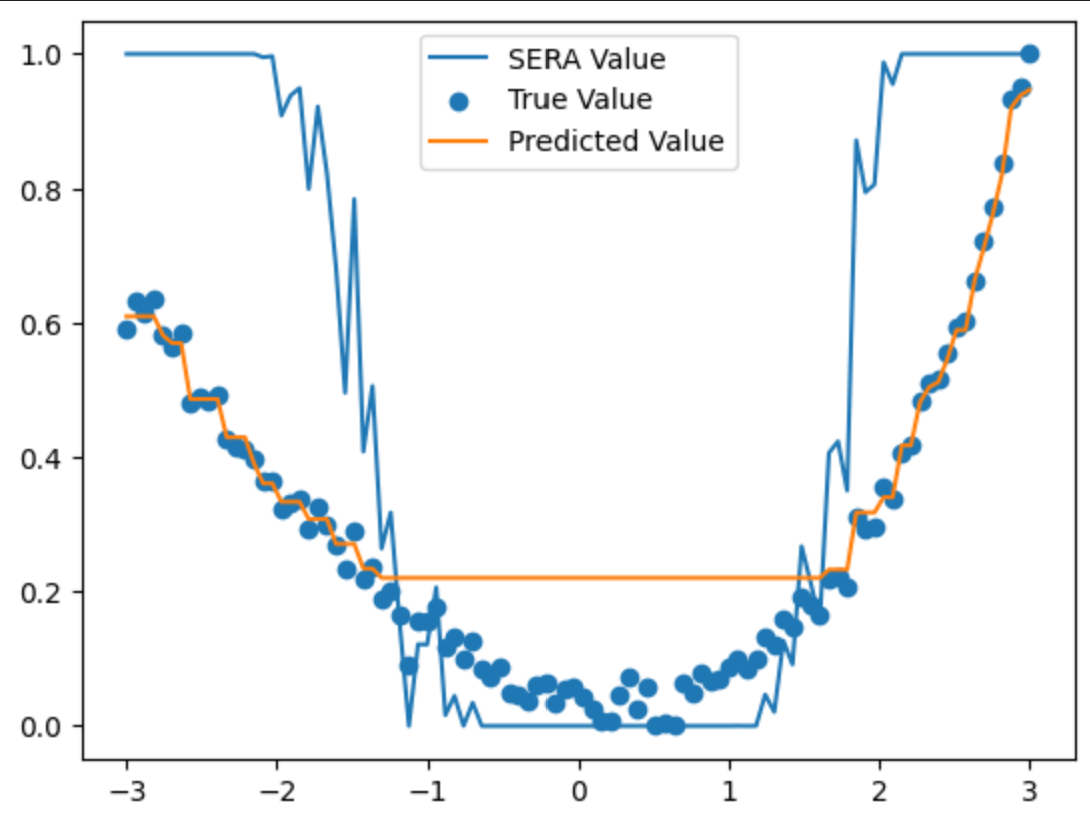
\includegraphics[width=0.7\linewidth]{assets/sera-loss-visualization.png}
    \caption{Visualization of the SERA loss and its effects}
    \label{fig:sera-loss-visualization}
\end{figure}
In this toy example it may seem like introducing the SERA loss only worsens the prediction. However, this is only due to the true function being an extremely easy one to fit and thus predict. With more complex functions, allowing the model to focus only on the parts of the distribution one deems more important can really help the model in the fitting of those sections. 

For the actual implementation of this loss function, note how many of the models mentioned in the \nameref{s:models} section are able to work with custom loss functions. However, to analyze whether a custom loss function helps in improving model accuracy for extreme values it is not necessary to retrain all models with this loss function. A single model will be trained with this loss function and its results will be compared to those obtained with the baseline loss function (MAE). The chosen model for the analysis has been the XGBoost given its ease of training and simplicity. In order to implement the $SERA$ loss function for the XGBoost library, functions defining its gradient and hessian have been created.
\subsection{Evaluation metrics}
\label{s:evaluation-metrics}
In order to understand why the following metrics have been chosen for evaluation it is important to keep in mind the overarching goal of the project. The goal of the mentioned models is not to provide an accurate short term forecast, but to provide a model that properly simulates the long term dynamics of the three time series. That is, models that are able of producing long term scenarios of solar and wind generation with univariate and multivariate dynamics equivalent to the real world ones, in order to optimize and test several grid planning possibilities on these scenarios. 

In order to best achieve this goal, the best performing model will have to be evaluated on different metrics, each corresponding to different attributes needed for correct whole picture modeling. These are the different attributes that will be tested and the metrics that will be used to test them. 

\subsubsection{Marginal distributions}
The first metric that will be evaluated will be the similarity of the univariate series with the real world data. Note that this similarity is not a point wise similarity. In many relevant papers, the accuracy of a series prediction is calculated through metrics like the RMSE or the MAPE. However, these metrics require that the prediction try to get right the value at each time step. If there is a delay of one time step, or a "cloudy week" comes a week earlier or later the RMSE will give a very poor score even though the general behavior is the same. That is why the approach taken here will be slightly different. The metrics used will be the following:
\begin{itemize}
    \item \textbf{Cramér von Mises criterion}: The Cramér von Mises criterion introduced by \cite{cramer_28} measures the distance between two CDF. It is calculated like:
    \begin{equation}
        \omega^2=\int_{-\infty}^{\infty}\left[F_m\left(x\right)-F_e\left(x\right)\right]^2dF_e\left(x\right)
    \end{equation}
    Where $F_m\left(x\right)$ is the modelled empirical CDF and $F_e\left(x\right)$ is the observed empirical CDF.
    \item \textbf{Kullback-Leibler divergence}: The KL divergence or relative entropy introduced in \cite{kullback_leibler_1951} is a statistical distance that measures how different a probability distribution is from another reference one. It is calculated like
    \begin{equation}
        D_{KL}\left(P||Q\right)=\sum_x P\left(x\right)\log{\left(\frac{P\left(x\right)}{Q\left(x\right)}\right)}
    \end{equation}
    where $P$ is the modelled probability distribution and Q is the reference probability distribution.

    In its implementation the probability distributions for the observed and predicted data are calculated through a kernel density estimate with a Gaussian kernel, as explained in the \nameref{s:individual-statistical-characteristics} section. The KL Divergence is then calculated on these PDFs.
    \item \textbf{ACF distance}: Even though the marginal distributions are by themselves a fundamental part of the closeness of the univariate series to reality, they are not the only one. Another key aspect of the series is its temporal self dependency, studied through the ACF of the correlation coefficient and the new correlation coefficient in the section called \nameref{sec:lagged-relationships}. The difference between the ACF of the $\xi$ metric of the empirical data and the model will be measured through a weighted root mean squared error, calculated as:
    \begin{equation}
        \text{ACFD}=\sqrt{\frac{\sum_{k=0}^N |w_k|\left[ACF_m\left(k\right)-ACF_e\left(k\right)\right]^2}{\sum_{k=0}^N |w_k|}}
    \end{equation}
    where $N$ is the number of periods for which the metric is calculated -- 72 in this case, $ACF_m$ is the model's $\xi$ ACF, $ACF_e$ is the empirical $\xi$ ACF and $w$ is the weighting factor, determined to be $w_k=ACF_e\left(k\right)$. This has been chosen so that a higher weight is given to those lags with a higher empirical relevance. 
    % \item \textbf{Seasonal metrics}: The metrics above will be calculated on the overall sample but also on subsamples divided by yearly season and daily period, to ensure the fit not only on a global scale but also on specific periods. 
\end{itemize}
\subsubsection{Joint distributions}
Now that it is clear how the marginal distributions will be assessed, it is time to look at how the dependence structure between the three series will be tested. There are several metrics that will be used for that purpose:
\begin{itemize}
    \item \textbf{Copula correlation matrix distance}: In the section regarding \nameref{sec:multivariate-analysis}, the correlation matrix of a Gaussian copula representing the dependence structure between the series was calculated. The same matrix will be calculated for samples of each of the models. Then, the distance (CCMD) between both matrices will be calculated. This distance is calculated as:
    \begin{equation}
        CCMD=\sqrt{\sum_i\sum_j\left(a_{ij}-b_{ij}\right)^2}
    \end{equation}
    where $A=\{a_{ij}\}$ is the correlation matrix of the copula fitted to the modelled data and $B=\{b_{ij}\}$ is the correlation matrix shown in \autoref{table:copula-correlation-matrix}.
    \item \textbf{CCF distance}: The cross correlation function distance is analogous to the autocorrelation function distance explained above, but for the $\xi$ cross correlation function instead of ACF.
    % \item \textbf{Seasonal metrics}: Similarly to the univariate case, the metrics above will be calculated on the whole period but also with seasonal differences and daily period differences.
\end{itemize}

\subsubsection{Extreme value analysis}
A significantly important aspect of the models is their need to be particularly accurate on the extreme values. Periods of extreme wind or solar generation are particularly interesting to the grid, due to their displacement of other energy sources or their need of them. That is why the accuracy of the models on extreme values will be assessed through these metrics:
\begin{itemize}
    % \item \textbf{Anderson-Darling statistic}:
    \item \textbf{Conditional Value at Risk distance}: The CVaR, usually used in financial risk management, measures what a certain value on average will be given that a certain threshold has been exceeded. It is calculated as 
    \begin{equation}
        \text{CVaR}_{\alpha}(x) = \mathbb{E} \left[X\mid X>\text{VaR}_{\alpha}\right]
    \end{equation} 
    with $\text{VaR}_{\alpha}$ being the Value at Risk for a given certainty. That is, the maximum value not exceeded with a probability $\alpha$. It is characterized as 
    \begin{equation}
        \text{VaR}_{\alpha}=\text{inf}\{x|F_X(x)\geq\alpha\}
    \end{equation}
    The assessment metric will be the difference between the modeled and empirical CVaR calculated as 
    \begin{equation}
        \text{CVRD}=\frac{\text{CVaR}^m_{95\%}}{\text{CVaR}^e_{95\%}}-1
    \end{equation}
    where $\text{CVaR}^m_{95\%}$ is the CVaR at a 95\% level for the model and $\text{CVaR}^e_{95\%}$ is the empirical CVaR at a 95\% level.
    \item \textbf{Tail dependence coefficient}: The tail dependence coefficient is a measure of the comovements of the tails of their distributions. It can be lower tail dependence or upper tail dependence, with the lower tail dependence calculated as 
    \begin{equation}
        \lambda_l=\lim_{q \to 0} P\left(X_m \leq F^{-1}_m(q) \mid X_e \leq F^{-1}_e(q)\right)  
    \end{equation}
    and the upper tail dependence coefficient being calculated as 
    \begin{equation}
        \lambda_u=\lim_{q \to 1} P\left(X_m > F^{-1}_m(q) \mid X_e > F^{-1}_e(q)\right)  
    \end{equation}
    with $F^{-1}_m$ being the inverse CDF for the model and $F^{-1}_e$ being the empirical inverse CDF.

    The tail dependence between each modeled variable with its corresponding empirical variable will be studied -- e.g. tail dependence between modeled solar PV with empirical solar PV.  

    Note how in practice there is not enough data to calculate an infinitesimally continuous $F^{-1}_m$ or $F^{-1}_e$. Therefore, an approximation will be done where instead of calculating the limit, the coefficient for a $q=0.05$ or $q=0.95$ -- depending on which tail is being studied -- will be used. 
    \item \textbf{Return level distance}: The GEV function is a function often used to model the maxima of sequences of random variables. Its CDF is
    \begin{equation}
        P\left(GEV\left(\mu,\sigma,\xi\right)\leq x\right)=e^{-t\left(x\right)}
    \end{equation}
    with
    \begin{equation}
        t\left(x\right)\equiv 
        \begin{cases} 
        \left[ 1 + \xi \left( \frac{x - \mu}{\sigma} \right) \right]^{- \frac{1}{\xi}}, & \text{if } \xi \neq 0, \\
        e^{\left( - \frac{x - \mu}{\sigma} \right)}, & \text{if } \xi = 0.
        \end{cases}
    \end{equation}
    As it can be seen from the formulation above the distribution of maximum values depends on three variables, with $\xi$ governing the tail behavior. Once the GEV distribution is fitted to the data, the return level can be estimated. The return level is the value expected to be exceeded on average once in a given period. If the 100-year return level of wind capacity factor is 0.95, that means that on average there will be one instance every 100 years when the capacity factor exceeds 0.95. The return level $z_T$ is calculated as 
    \begin{equation}
        z_T=\mu+\frac{\sigma}{\xi}\left[\left(-\text{log}\left(1-\frac{1}{T}\right)\right)^{-\xi}-1\right]
    \end{equation}
    Thus, the weekly maxima will be obtained with the data, with which a GEV distribution will be fitted and a 10-year return level will be calculated. The assessment metric will be the percentage difference in return level calculated as 
    \begin{equation}
        \text{RLD}=\frac{z^m_{10}}{z^e_{10}}-1
    \end{equation}
    This will be calculated for both the maxima and the minima of the distributions. 
\end{itemize}

The extreme value assessment is particularly important for wind generation, rather than for solar generation as it is much more consistent. Therefore, these values will only be calculated for the wind series. 

\subsection{Model training and validation}
\label{s:model-training-and-validation}
After having laid out the different evaluation metrics that will be used, the method used for training and validating the models will be presented. 

A general train-test-validation split will be used. This approach splits the available data in three groups. The first will be used to train the models. The second will be used to test the models and iteratively improve these models, by checking for overfitting and evaluating different parameter setups. The validation data is left as the final evaluation data, where the final metrics that will be presented are calculated. The metrics obtained in this group can be seen as the metrics that are to be expected of the models in a real world context after deployment. A split of 1 year validation data, 1 year testing data and the rest as training data has been chosen, as a 1-year prediction horizon is a long enough horizon to test the long run characteristics of the model and it contains values for all different seasons. 

As it can be seen in the \nameref{s:evaluation-metrics} section there are many evaluation metrics attempting to check for different characteristics of the model. Therefore, using a programmatic approach to model creating through something like a grid search of parameters is not really useful, as it can be difficult to determine in an algorithmic way which results are better than others, as one model can have better results modeling extreme values while others can have better results in modeling cross relationships. Therefore, a manual approach to model improvement with the test set will be employed, and only the best overall model selected in a discretionary way will be evaluated on the validation set and will have its results presented in this work.

Another thing worth mentioning is that no cross validation or bootstrapping methods will be used to evaluate the models. Although these approaches would give a more robust understanding of the validity of the model by being more resistant to anomalies in the test and validation sets, the amount of data available for training -- specially for the neural network and transformer based models -- is not enough in order to sacrifice even more for testing and validation purposes.

As an alternative approach to cross validation and bootstrapping, the test and validation sets will be evaluated for anomalies. That is, they will be evaluated as if they were a prediction against the previous year. The results are the following:

\begin{table}[ht]
    \centering
    \begin{tabular}{rll}
        \toprule
        \textbf{Solar PV} & \multicolumn{2}{c}{Period} \\ 
        \cmidrule(lr){2-3}
            & Test & Validation \\
        \midrule
        Cramer von Mises & 29.34 & 9.48 \\
        KL divergence & 0.0003 & 0.0004 \\
        ACF$_\xi$ distance & 0.0127 & 0.0137 \\
        \midrule
        CCMD & 0.0112 & 0.0167 \\
        CCF$_\xi^{Solar TH}$ distance & 0.0099 & 0.0338\\
        CCF$_\xi^{Wind}$ distance & 0.0119 & 0.0372 \\
        \midrule
        CVaR$^+$ distance & -0.0297 & -0.0064 \\
        % CVaR$^-$ distance & 0.8416 & -0.2067 \\
        Tail dependence coefficient$^+$ & 0.3676 & 0.4703 \\
        % Tail dependence coefficient$^-$ & 0.1119 & 0.1381 \\
        Return level distance$^+$ & 0.0154 & -0.0248 \\
        % Return level distance$^-$ & 0.0289 & -0.0661 \\
        \bottomrule
    \end{tabular}
    \caption{Evaluation metrics of the test and validation sets with respect to the previous year for solar PV}
    \label{table:eval-metrics-test-validation-solar-pv}
\end{table}

At a first glance it can be seen how some metrics seem to be more consistent than others. The Cramer von Mises statistic for example exhibits what seems to be a great difference between one and the other year, while the KL divergence seems to be more reliable exhibiting a much lesser difference. These values will be useful as they represent a baseline of what a reasonable \textit{error} according to the different metrics would be. If when evaluating a model the metric is similar to the ones shown here, the predicted values can be approximated to be close enough to what a the real process would generate. 

Note how for solar PV the metrics regarding the extreme values in the left tail have been left out, as the values here are very close to zero and thus these metrics are very noisy. The same will be done for solar TH. 

\begin{table}[ht]
    \centering
    \begin{tabular}{rll}
        \toprule
        \textbf{Solar TH} & \multicolumn{2}{c}{Period} \\ 
        \cmidrule(lr){2-3}
            & Test & Validation \\
        \midrule
        Cramer von Mises & 12.86 & 9.89 \\
        KL divergence & 0.0102 & 0.0265 \\
        ACF$_\xi$ distance & 0.0249 & 0.0162 \\
        \midrule
        CCMD & 0.0112 & 0.0167 \\
        CCF$_\xi^{Solar PV}$ distance & 0.0151 & 0.0155 \\
        CCF$_\xi^{Wind}$ distance & 0.0201 & 0.0229 \\
        \midrule
        CVaR$^+$ distance & 0.0732 & -0.1318 \\
        % CVaR$^-$ distance & 0.8416 & -0.2067 \\
        Tail dependence coefficient$^+$ & 0.3356 & 0.2968 \\
        % Tail dependence coefficient$^-$ & 0.1119 & 0.1381 \\
        Return level distance$^+$ & 0.2928 & -0.1504 \\
        % Return level distance$^-$ & 0.0289 & -0.0661 \\
        \bottomrule
    \end{tabular}
    \caption{Evaluation metrics of the test and validation sets with respect to the previous year for solar TH}
    \label{table:eval-metrics-test-validation-solar-th}
\end{table}

In \autoref{table:eval-metrics-test-validation-solar-th} the same metrics shown before but for solar TH can be seen. Again, these will be used as benchmarks for the modeling of solar thermal by the different models. Note how the CCMD metrics are the same, as the copula matrix is the same one for all three series, and the distance is thus also equivalent.

\begin{table}[ht]
    \centering
    \begin{tabular}{rll}
        \toprule
        \textbf{Wind} & \multicolumn{2}{c}{Period} \\ 
        \cmidrule(lr){2-3}
            & Test & Validation \\
        \midrule
        Cramer von Mises & 9.48 & 5.01 \\
        KL divergence & 0.0.0018 & 0.0018 \\
        ACF$_\xi$ distance & 0.0602 & 0.0630 \\
        \midrule
        CCMD & 0.0112 & 0.0167 \\
        CCF$_\xi^{Solar PV}$ distance & 0.0128 & 0.0111 \\
        CCF$_\xi^{Solar TH}$ distance & 0.0136 & 0.0131 \\
        \midrule
        CVaR$^+$ distance & -0.0236 & -0.0016 \\
        CVaR$^-$ distance & -0.2461 & 0.2123 \\
        Tail dependence coefficient$^+$ & 0.0479 & 0.2443 \\
        Tail dependence coefficient$^-$ & 0.1506 & 0.1119 \\
        Return level distance$^+$ & 1.3618 & -0.0071 \\
        Return level distance$^-$ & -13.5111 & -1.1904 \\
        \bottomrule
    \end{tabular}
    \caption{Evaluation metrics of the test and validation sets with respect to the previous year for wind}
    \label{table:eval-metrics-test-validation-wind}
\end{table}

Finally, in \autoref{table:eval-metrics-test-validation-wind} the same metrics that will be used as benchmarks for wind can be seen. Here, the metrics relating to the extremes in the negative tail have been included since for wind it does hold some interest to see whether the model accurately models periods of low wind generation.